\documentclass[letter,twoside,11pt]{article}

\usepackage[spanish,es-nodecimaldot]{babel}
\usepackage[utf8]{inputenc}

\usepackage{lmodern}
\usepackage[T1]{fontenc}
\usepackage{textcomp}

\usepackage{framed}
\usepackage[svgnames]{xcolor}
\colorlet{shadecolor}{Gainsboro!50}

\usepackage[labelfont=bf]{caption}
\usepackage{graphicx}
\usepackage{pstricks}

\usepackage{anysize}
\marginsize{3cm}{2cm}{2cm}{3cm}

\usepackage{siunitx}
\usepackage{amsmath}
\usepackage{array}
\usepackage{csquotes}

\usepackage{fancyhdr}
\usepackage{lastpage}
\pagestyle{fancy}
\fancyhf{}
\fancyhead[LE,RO]{Laboratorio de Electrónica Analógica I}
\fancyfoot[CO,CE]{\thepage\ de \pageref{LastPage}}

\special{papersize=215.9mm,279.4mm}

\usepackage[
    pdfauthor={Carlos Eduardo Caballero Burgoa},%
    pdftitle={Laboratorio de Electrónica Analógica I},%
    pdfsubject={Curva de polarización, recortadores y sujetadores},%
    colorlinks,%
    citecolor=black,%
    filecolor=black,%
    linkcolor=black,%
    urlcolor=black,
    breaklinks]{hyperref}
\usepackage{breakurl}

\newcommand{\blankpage}{
\newpage
\thispagestyle{empty}
\mbox{}
\newpage
}

\renewcommand{\arraystretch}{1.2}

\begin{document}

\begin{titlepage}
    \begin{center}
        {\Large UNIVERSIDAD MAYOR DE SAN SIMÓN}\\
        \vspace*{0.15cm}
        {\large FACULTAD DE CIENCIAS Y TECNOLOGÍA}\\
        \vspace*{0.10cm}
        DEPARTAMENTO DE ELÉCTRICA-ELECTRÓNICA\\
        \vspace*{3.0cm}
        {\Large \textbf{LABORATORIO DE ELECTRÓNICA ANALÓGICA I}}\\
        \vspace*{0.3cm}
        {\Large \textbf{INFORME No. 1}}\\
        \vspace*{3.5cm}
        {\Large \textbf{CURVA DE POLARIZACIÓN,\\RECORTADORES Y SUJETADORES}}\\
    \end{center}

    \vspace*{5.8cm}
    \leftskip=7.95cm
    \noindent
    \textbf{Estudiante:}\\
    Caballero Burgoa, Carlos Eduardo.\\
    \newline
    \textbf{Carrera:}\\
    Ing. Electromecánica.\\
    \newline
    \textbf{Docente:}\\
    Ing. Alberto Arispe Santander.\\
    \newline
    \textbf{Grupo:} 1B.\\
    \textbf{Fecha de entrega:} 1 de Octubre del 2024.\\
\end{titlepage}

\section{Objetivos}
\begin{itemize}
    \item Verificar la curva caracteristica de polarización de un diodo.
    \item Verificar el comportamiento de circuitos recortadores.
    \item Verificar el comportamiento de circuitos sujetadores.
\end{itemize}

\section{Marco Teorico}
El dispositivo electrónico no lineal más simple se conoce como \emph{diodo}. Un
diodo está compuesto de dos materiales diferentes colocados juntos de tal forma
que la carga fluye fácilmente en una dirección, pero no en dirección contraria.
\cite{Savant}

\subsection{Curva caracteristicas de polarización}
En la figura (\ref{curva}), se muestra la grafica de la corriente en funcion del
voltaje, donde pueden observarse tres regiones donde puede operar el diodo:
\cite{Tankara}

\begin{description}
    \item [Region de conduccion en polarizacion directa (PD)]
        Donde $V_D > 0[V]$, siendo:
        \begin{itemize}
            \item La corriente en el diodo muy pequeña, cuando $0[V] < V_D < V_F$.
            \item La corriente en el diodo es cada vez mas grande, cuando $V_D > V_F$.
        \end{itemize}
    \item [Region de no conducción]
        Donde $V_D < 0[V]$, siendo la corriente en el diodo demasiado pequeña y
        negativa, conocida como corriente de saturacion inversa: $I_S$.
    \item [Region de conduccion en polarizacion inversa]
        Se encuentra a la izquierda del voltaja de ruptura $V_{BR}$, para
        voltajes del diodo cada vez mayor, pero negativo, el diodo se encuentra
        con corriente cada vez mas grande (pero negativa), conocida como
        corriente de avalancha.
\end{description}

\subsection{Circuito recortadorl

\section{Simulación}
Se utilizó el software \emph{Quite Universal Circuit Simulator.} version 23.3.1
para simular los circuitos.

\subsection{Curva de polarización}
La curva de polarización simulada para dos diodos en serie puede verse en la
figura (\ref{simulacion1}):

\begin{figure}[!h]
\centering
\includegraphics[scale=1.00]{simulacion/practica1.1.eps}
\caption{Simulación de la curva V-I en dos diodos en serie.}
\label{simulacion1}
\end{figure}

\subsection{Recortador sin fuente de voltaje}
Se simulo un circuito recortador con tres tipos diferentes de señales: una señal
rectangular (\ref{simulacion2}), una señal triangular (\ref{simulacion3}) y una
señal sinusoidal (\ref{simulacion4}).

\begin{figure}[!h]
\centering
\includegraphics[scale=1.00]{simulacion/practica1.2.eps}
\caption{Simulación de un recortador con una señal rectangular.}
\label{simulacion2}
\end{figure}

\begin{figure}[!h]
\centering
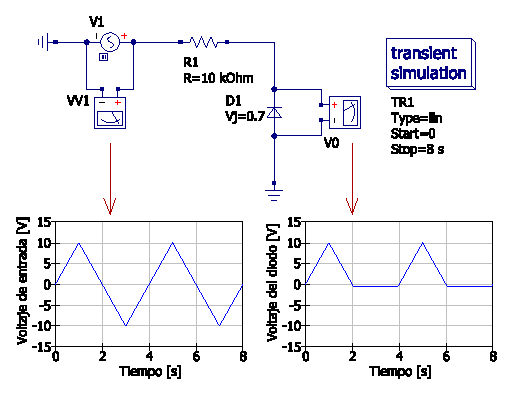
\includegraphics[scale=1.00]{simulacion/practica1.3.eps}
\caption{Simulación de un recortador con una señal triangular.}
\label{simulacion3}
\end{figure}

\begin{figure}[!h]
\centering
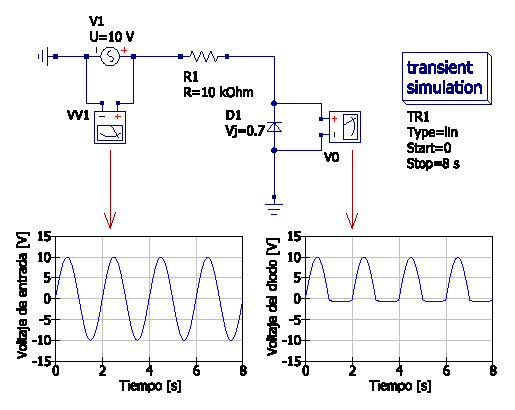
\includegraphics[scale=1.00]{simulacion/practica1.4.eps}
\caption{Simulación de un recortador con una señal senoidal.}
\label{simulacion4}
\end{figure}

\subsection{Recortador con fuente de voltaje}
Se simulo un circuito recortador con fuente de voltaje de $5[V]$  con tres tipos
diferentes de señales: una señal rectangular (\ref{simulacion5}), una señal
triangular (\ref{simulacion6}) y una señal sinusoidal (\ref{simulacion7}).

\begin{figure}[!h]
\centering
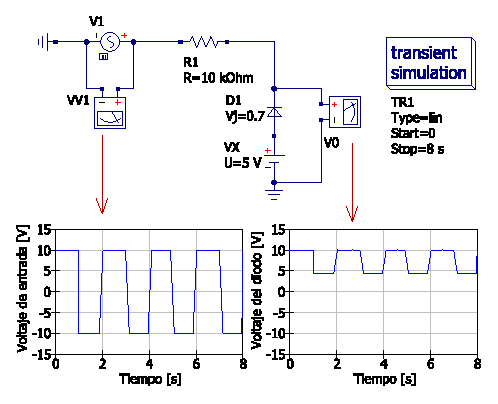
\includegraphics[scale=1.00]{simulacion/practica1.5.eps}
\caption{Simulación de un recortador con fuente de voltaje con una señal rectangular.}
\label{simulacion5}
\end{figure}

\begin{figure}[!h]
\centering
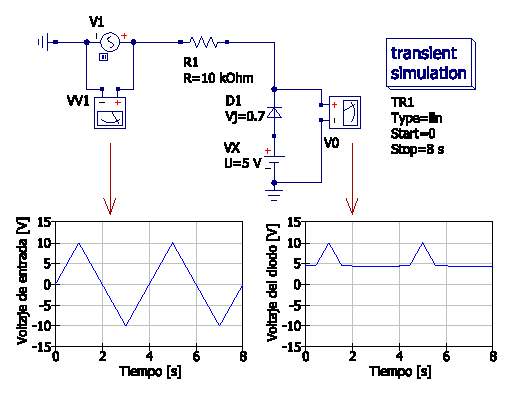
\includegraphics[scale=1.00]{simulacion/practica1.6.eps}
\caption{Simulación de un recortador con fuente de voltaje con una señal triangular.}
\label{simulacion6}
\end{figure}

\begin{figure}[!h]
\centering
\includegraphics[scale=1.00]{simulacion/practica1.7.eps}
\caption{Simulación de un recortador con fuente de voltaje con una señal senoidal.}
\label{simulacion7}
\end{figure}

\subsection{Sujetador sin fuente de voltaje}
Se simulo un circuito sujetador con tres tipos diferentes de señales: una señal
rectangular (\ref{simulacion8}), una señal triangular (\ref{simulacion9}) y una
señal sinusoidal (\ref{simulacion10}).

\begin{figure}[!h]
\centering
\includegraphics[scale=1.00]{simulacion/practica1.8.eps}
\caption{Simulación de un sujetador con una señal rectangular.}
\label{simulacion8}
\end{figure}

\begin{figure}[!h]
\centering
\includegraphics[scale=1.00]{simulacion/practica1.9.eps}
\caption{Simulación de un sujetador con una señal triangular.}
\label{simulacion9}
\end{figure}

\begin{figure}[!h]
\centering
\includegraphics[scale=1.00]{simulacion/practica1.10.eps}
\caption{Simulación de un sujetador con una señal senoidal.}
\label{simulacion10}
\end{figure}

\subsection{Sujetador con fuente de voltaje}
Se simulo un circuito sujetador con fuente de voltaje de $5[V]$  con tres tipos
diferentes de señales: una señal rectangular (\ref{simulacion11}), una señal
triangular (\ref{simulacion12}) y una señal sinusoidal (\ref{simulacion13}).

\begin{figure}[!h]
\centering
\includegraphics[scale=1.00]{simulacion/practica1.11.eps}
\caption{Simulación de un sujetador con fuente de voltaje con una señal rectangular.}
\label{simulacion11}
\end{figure}

\begin{figure}[!h]
\centering
\includegraphics[scale=1.00]{simulacion/practica1.12.eps}
\caption{Simulación de un sujetador con fuente de voltaje con una señal triangular.}
\label{simulacion12}
\end{figure}

\begin{figure}[!h]
\centering
\includegraphics[scale=1.00]{simulacion/practica1.13.eps}
\caption{Simulación de un sujetador con fuente de voltaje con una señal senoidal.}
\label{simulacion13}
\end{figure}

\section{Resultados}

\subsection{Curva de polarización}
En laboratorio de se obtuvieron los siguientes datos:

\begin{center}
    \begin{tabular}{|c|c|c|}
    \hline
    $V_i [V]$ & $V_d [V]$ & $i [A]$
    \tabularnewline \hline \hline
    $0.4$ & $0.29$ & $0.001$ \tabularnewline \hline
    $1$   & $0.80$ & $0.014$ \tabularnewline \hline
    $2$   & $0.95$ & $0.094$ \tabularnewline \hline
    $3$   & $1.02$ & $0.188$ \tabularnewline \hline
    $4$   & $1.06$ & $0.286$ \tabularnewline \hline
    $5$   & $1.08$ & $0.379$ \tabularnewline \hline
    \end{tabular}
\end{center}

\section{Conclusiones y Recomendaciones}

\begin{thebibliography}{99}

\bibitem{Savant}
C.J. Savant Jr, Martin S. Roden, Gordon Carpenter. (1992).\\
\textbf{Diseño Electrónico. Circuitos y sistemas. 2da Edición.}\\
Addison-Wesley

\bibitem{Tancara}
Ing. Jose F. Tancara S. (2019).\\
\textbf{Guia de laboratorio electronica analogica I}\\

%\bibitem{DTO} Dual Trace Oscilloscope. User Manual \\
%Extraído el 16 de Septiembre del 2024, de: \\
%\url{https://www.gwinstek.com/en-IN/products/detail/GOS-630FC}

\end{thebibliography}

\end{document}

